% \section*{RISC-V Instruction Set}
\begin{tabbing}
    Base format: \quad \= \texttt{Inst rd, rs1, rs2} (\texttt{rd}: destination register, \texttt{rs1, rs2} source registers).\\
    Other formats: \> \texttt{Inst rs1, rs2}\\
    \> \texttt{Inst rs1, immediate}
\end{tabbing}

\begin{multicols}{2}
\textbf{RV32I Base Integer Instructions}\\
        \begin{tabular}
        {| T | l | l |} \hline
        \rm Inst & Name                    & \rm Description (C)          \\ \hline
        add      & ADD                     & rd = rs1 + rs2               \\
        sub      & SUB                     & rd = rs1 - rs2               \\
        xor      & XOR                     & rd = rs1 \^{} rs2            \\
        or       & OR                      & rd = rs1 | rs2               \\
        and      & AND                     & rd = rs1 \& rs2              \\
        sll      & Shift Left Logical      & rd = rs1 \verb|<<| rs2       \\
        srl      & Shift Right Logical     & rd = rs1 \verb|>>| rs2       \\
        sra      & Shift Right Arith*      & rd = rs1 \verb|>>| rs2       \\
        slt      & Set Less Than           & rd = (rs1 < rs2)?1:0         \\
        sltu     & Set Less Than (U)       & rd = (rs1 < rs2)?1:0         \\ \hline
        addi     & ADD Immediate           & rd = rs1 + imm               \\
        xori     & XOR Immediate           & rd = rs1 \^{} imm            \\
        ori      & OR Immediate            & rd = rs1 | imm               \\
        andi     & AND Immediate           & rd = rs1 \& imm              \\
        \end{tabular}
        \begin{tabular}
        {| T | l | l |} \hline
        slli     & Shift Left Logical Imm  & rd = rs1 \verb|<<| imm[0:4]  \\
        srli     & Shift Right Logical Imm & rd = rs1 \verb|>>| imm[0:4]  \\
        srai     & Shift Right Arith Imm   & rd = rs1 \verb|>>| imm[0:4]  \\
        slti     & Set Less Than Imm       & rd = (rs1 < imm)?1:0         \\
        sltiu    & Set Less Than Imm (U)   & rd = (rs1 < imm)?1:0         \\ \hline
        lb       & Load Byte               & rd = M[rs1+imm][0:7]         \\
        lh       & Load Half               & rd = M[rs1+imm][0:15]        \\
        lw       & Load Word               & rd = M[rs1+imm][0:31]        \\
        lbu      & Load Byte (U)           & rd = M[rs1+imm][0:7]         \\
        lhu      & Load Half (U)           & rd = M[rs1+imm][0:15]        \\ \hline
        sb       & Store Byte              & M[rs1+imm][0:7]  = rs2[0:7]  \\
        sh       & Store Half              & M[rs1+imm][0:15] = rs2[0:15] \\
        sw       & Store Word              & M[rs1+imm][0:31] = rs2[0:31] \\ \hline
        beq      & Branch ==               & if(rs1 == rs2) PC += imm     \\
        bne      & Branch !=               & if(rs1 != rs2) PC += imm     \\
        blt      & Branch <                & if(rs1 < \enspace rs2) PC += imm \\
        bge      & Branch $\leq$           & if(rs1 >= rs2) PC += imm     \\
        bltu     & Branch < (U)            & if(rs1 < \enspace rs2) PC += imm \\
        bgeu     & Branch $\geq$ (U)       & if(rs1 >= rs2) PC += imm     \\ \hline
        jal      & Jump And Link           & rd = PC+4; PC += imm         \\
        jalr     & Jump And Link Reg       & rd = PC+4; PC = rs1 + imm    \\ \hline
        lui      & Load Upper Imm          & rd = imm \verb|<<| 12        \\
        auipc    & Add Upper Imm to PC     & rd = PC + (imm \verb|<<| 12) \\ \hline
        ecall    & Environment Call        & Transfer control to OS       \\ \hline
        ebreak   & Environment Break       & Transfer control to debugger \\ \hline
        \end{tabular}

        
\columnbreak

\textbf{Registers}\\
\begin{tabular} {|l | l | l | l|} \hline
Register     & ABI Name     & Description           & Saver  \\ \hline
\tt{x0}      & \tt{zero}    & Zero constant         & ---    \\
\tt{x1}      & \tt{ra}      & Return address        & Caller \\
\tt{x2}      & \tt{sp}      & Stack pointer         & ---    \\
\tt{x3}      & \tt{gp}      & Global pointer        & ---    \\
\tt{x4}      & \tt{tp}      & Thread pointer        & Callee \\
\tt{x5-x7}   & \tt{t0-t2}   & Temporaries           & Caller \\
\tt{x8}      & \tt{s0 / fp} & Saved / frame pointer & Callee \\
\tt{x9}      & \tt{s1}      & Saved register        & Callee \\
\tt{x10-x11} & \tt{a0-a1}   & Fn args/return values & Caller \\
\tt{x12-x17} & \tt{a2-a7}   & Fn args               & Caller \\
\tt{x18-x27} & \tt{s2-s11}  & Saved registers       & Callee \\
\tt{x28-x31} & \tt{t3-t6}   & Temporaries           & Caller \\ \hline
\end{tabular}

\vspace{10ex}
\begin{flushright}
    \textbf{Calling convention stack layout$\qquad$}
    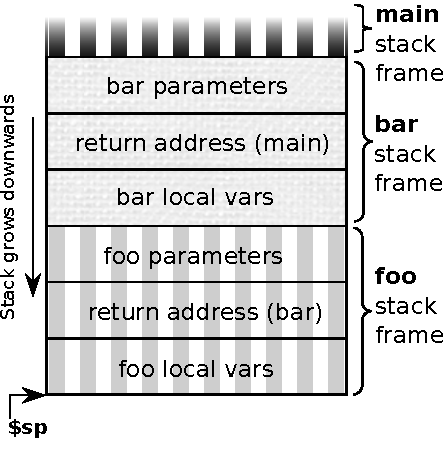
\includegraphics[width=0.35\textwidth]{img/call_stack_diagram.pdf}
\end{flushright}
    
\end{multicols}


\begin{multicols}{2}
    
    \textbf{RV32M Multiply Extension}\\
    \begin{tabular}
        {|T | l | c | T | T | T | C } \hline
        \rm Inst & Name              & \rm Description (C)     \\ \hline
        mul      & MUL               & rd = (rs1 * rs2)[31:0]  \\
        mulh     & MUL High          & rd = (rs1 * rs2)[63:32] \\
        mulsu    & MUL High (S) (U)  & rd = (rs1 * rs2)[63:32] \\
        mulu     & MUL High (U)      & rd = (rs1 * rs2)[63:32] \\
        div      & DIV               & rd = rs1 / rs2          \\
        divu     & DIV (U)           & rd = rs1 / rs2          \\
        rem      & Remainder         & rd = rs1 \% rs2         \\
        remu     & Remainder (U)     & rd = rs1 \% rs2         \\
        \hline
    \end{tabular}

    \columnbreak

    \textbf{C compiler datatype sizes}\\
    \begin{tabular} {|l | l | l |} \hline
        C type              &  Description             & Bytes in RV32      \\ \hline
        \texttt{char}       & Character value/byte     & 1                  \\
        \texttt{short}      & Short integer            & 2                  \\
        \texttt{int}        & Integer                  & 4                  \\
        \texttt{long}       & Long integer             & 4                  \\
        \texttt{long long}  & Long long integer        & 8                  \\
        \texttt{void*}      & Pointer                  & 4                  \\
        \texttt{float}      & Single-precision float   & 4                  \\
        \texttt{double}     & Double-precision float   & 8                  \\
        \texttt{long double}& Extended-precision float & 16                 \\\hline
    \end{tabular}
\end{multicols}